\chapter{Von der lokalen Erhaltung zu Einsteins Feldgleichungen}

Einsteins Feldgleichungen lassen sich einfach in einer Zeile hinschreiben, sind aber notorisch unangenehm in Komponentenform auszurechnen. Eine Metrik hat viele Christoffel-Symbole; die Christoffel-Symbole enthalten Ableitungen der Metrik; und der Krümmungstensor enthält sowohl Ableitungen als auch Produkte von Christoffel-Symbolen. Schon bevor man versucht, irgendetwas zu lösen, kann die Rechnung Seiten füllen. Für eine bestimmte Metrik ist symbolische Software oft das geeignete Mittel, um diese Buchführung zu bewältigen.

Die Prinzipien sind viel klarer als die Rechnung. Deshalb beginnen wir nicht damit, die Gleichungen Komponente für Komponente anzugehen. Wir fragen, welche Art von Gleichung die Gravitation erfordert. Die Argumentation geht von der Newtonschen Theorie aus, führt über die lokale Erhaltung und endet mit der Entdeckung jener Kombination von Krümmungstensoren, die konsistent dem Fluss und der Dichte von Energie und Impuls gleichgesetzt werden kann. Im gesamten Kapitel verwenden wir \(c=1\).

\section{Die Newtonsche Wechselwirkung in beide Richtungen}

Die Gravitation gibt zwei einander ergänzende Anweisungen. Das Gravitationsfeld sagt der Materie, wie sie sich bewegen soll, während die Materie dem Gravitationsfeld vorgibt, wie es beschaffen sein soll. Diese Wechselwirkung in beide Richtungen ist bereits in der Newtonschen Mechanik erkennbar.

Sei \(\phi(\mathbf{x},t)\) das Newtonsche Gravitationspotential. Auf einen Probekörper der Masse \(m\) wirkt die Kraft
\begin{equation}
 \mathbf{F}=-m\nabla\phi.
\end{equation}
Zusammen mit \(\mathbf{F}=m\mathbf{a}\) ergibt sich nach Kürzen der Probemasse:
\begin{equation}
 \mathbf{a}=-\nabla\phi.
\end{equation}
Dies ist die erste Richtung der Wechselwirkung. Ist das Feld bekannt, gibt es jedem frei fallenden Körper seine Beschleunigung vor, unabhängig von dessen Masse.

Die umgekehrte Richtung wird durch die Poisson-Gleichung beschrieben,
\begin{equation}
 \nabla^2\phi=4\pi G\rho,
 \qquad
 \nabla^2=
 \frac{\partial^2}{\partial x^2}
 +\frac{\partial^2}{\partial y^2}
 +\frac{\partial^2}{\partial z^2},
 \label{eq:poisson}
\end{equation}
wobei \(\rho(\mathbf{x},t)\) die Masse pro Volumeneinheit ist. Der Faktor \(4\pi\) könnte in die Definition von \(G\) aufgenommen werden, würde dann aber nur an anderer Stelle wieder auftauchen. Gleichung~\eqref{eq:poisson} besagt, dass die Materieverteilung die Quelle des Potentials ist.

Für einen kugelsymmetrischen Körper mit der Gesamtmasse \(M\) lautet die äußere Lösung
\begin{equation}
 \phi(r)=-\frac{GM}{r}.
 \label{eq:newton-potential}
\end{equation}
Die Dichte kann sich im Zentrum konzentrieren, gleichmäßig verteilt sein oder zum Rand hin stetig abnehmen. Die äußere Lösung hängt nur von der Kugelsymmetrie und der Gesamtmasse ab. Außerhalb der Materie gilt \(\nabla^2\phi=0\); durch Ableiten von \(1/r\) erhält man dann die Kraft mit umgekehrt quadratischem Abstandsgesetz. Betrachtet man nur den Außenbereich, kann man die Quelle zu einem Punkt schrumpfen und denselben Ausdruck überall außer an diesem Punkt verwenden.

\begin{classroomqa}
\audiencequestion{Muss die Dichte im Inneren des kugelförmigen Körpers konstant sein und an seiner Grenze sprunghaft auf null abfallen?}
\lecturerresponse{Nein. Für diese Argumentation muss sie kugelsymmetrisch sein, aber sie muss weder konstant sein noch einen Sprung aufweisen. Sie kann stetig auf null abnehmen. Keine dieser Einzelheiten im Inneren verändert das äußere Potential, das nur von der Gesamtmasse abhängt.
\lecturetimestamp{00:09:13--00:09:37}}
\end{classroomqa}

Diese Feldbeschreibung wirkt lokaler als eine direkte Kraft zwischen weit voneinander entfernten Massen, doch die Newtonsche Gravitation enthält weiterhin eine momentane Fernwirkung. Bewegt man die Quelle, ändert sich das Newtonsche Potential überall zugleich. Die allgemeine Relativitätstheorie muss neben dem Kraftgesetz auch diese momentane Reaktion ersetzen.

\section{Ein Hinweis aus dem schwachen Feld, noch keine Gleichung}

Die relativistische Fassung der ersten Anweisung kennen wir bereits: Ist die Raumzeitmetrik gegeben, folgen frei fallende Teilchen Raumzeitgeodäten. Nun brauchen wir den relativistischen Ersatz für die Poisson-Gleichung, also die Vorschrift, nach der die Materie die Metrik bestimmt.

Die Schwarzschild-Geometrie liefert einen Hinweis. Ihre Zeit-Zeit-Komponente lautet
\begin{equation}
 g_{00}=1-\frac{2GM}{r}.
\end{equation}
Mit Gleichung~\eqref{eq:newton-potential} wird daraus
\begin{equation}
 g_{00}=1+2\phi.
\end{equation}
Folglich gilt
\begin{equation}
 \nabla^2g_{00}=2\nabla^2\phi=8\pi G\rho.
 \label{eq:weak-mnemonic}
\end{equation}

Gleichung~\eqref{eq:weak-mnemonic} ist mit Vorsicht zu betrachten. Sie ist eine Merkhilfe, nicht Einsteins Gleichung. Sie verwendet eine ausgezeichnete Komponente der Metrik und eine nichtrelativistische Quelle. Dennoch zeigt sie die gesuchte Struktur: Auf der einen Seite steht eine Materiedichte, auf der anderen stehen zweite Ableitungen der Geometrie. Sie bildet die grobe Brücke von der Poisson-Gleichung zu einer kovarianten Feldgleichung.

Die rechte Seite muss nun genauer betrachtet werden. In relativistischen Einheiten ist Masse Energie, daher ist \(\rho\) zunächst als Energiedichte zu verstehen. Eine Energiedichte ist jedoch kein vollständiges relativistisches Objekt. Um zu sehen, was noch dazugehört, beginnen wir mit einer einfacheren Erhaltungsgröße.

\section{Ladungsdichte, Strom und lokale Erhaltung}

Sei \(Q\) die elektrische Ladung und \(\sigma\) die Ladungsdichte:
\begin{equation}
 \sigma=\lim_{\Delta V\to0}\frac{\Delta Q}{\Delta V}.
\end{equation}
Die Dichte gibt an, wie viel Ladung sich zu einem bestimmten Zeitpunkt in einem kleinen räumlichen Volumen befindet. Der Strom beantwortet eine andere Frage. Man stelle sich ein infinitesimal kleines, orientiertes Fenster im Raum vor und zähle, wie viel Ladung es pro Flächeneinheit und Zeiteinheit durchquert. Die drei möglichen Orientierungen ergeben die räumlichen Stromkomponenten \(J^i\).

Der Vergleich der Dimensionen ist aufschlussreich. Die Ladungsdichte ist die Ladung geteilt durch drei räumliche Längen. Der Strom ist die Ladung geteilt durch zwei räumliche Längen und ein Zeitintervall. Für \(c=1\) haben Zeit und Länge dieselben Einheiten, sodass Dichte und Strom übereinstimmende Dimensionen haben. Sie bilden zusammen einen Vierervektor:
\begin{equation}
 J^\mu=(J^0,J^1,J^2,J^3),
 \qquad J^0=\sigma.
\end{equation}

Ladungserhaltung bedeutet nicht bloß, dass die Gesamtladung im Universum konstant bleibt. Sie gilt lokal. Ladung kann nicht aus dem Hörsaal verschwinden und augenblicklich bei Alpha Centauri wieder auftauchen. Verlässt sie ein Gebiet, muss sie dessen Grenze überqueren. Bei einem kleinen Kasten entspricht die Abnahme der darin enthaltenen Ladung dem nach außen gerichteten Fluss durch seine Wände. Der Satz von Gauss ergibt
\begin{equation}
 \dot{\sigma}+\nabla\cdot\mathbf{J}=0,
\end{equation}
oder, in Summenkonvention geschrieben,
\begin{equation}
 \partial_\mu J^\mu=0.
 \label{eq:charge-continuity}
\end{equation}
In gekrümmten Koordinaten schreibt man die entsprechende Tensorgleichung mit einer kovarianten Ableitung:
\begin{equation}
 D_\mu J^\mu=0.
\end{equation}
Die kovariante Ableitung dient nicht der Ausschmückung. Sie macht die Aussage in jedem Koordinatensystem sinnvoll.

\section{Warum Energie und Impuls zwei Indizes benötigen}

Die Ladung selbst ist invariant. Beobachter, die sich relativ zueinander bewegen, stimmen über die Ladung eines Elektrons überein, auch wenn sie sich nicht über Ladungsdichte und Strom einig sind. Ein bewegter Beobachter sieht längenkontrahierte Volumina und möglicherweise einen Ladungsstrom, während ein anderer Beobachter die Ladungen als ruhend wahrnimmt. Bei einem Bezugssystemwechsel mischen sich daher Dichte und Strom, obwohl die Gesamtladung gleich bleibt.

Energie und Impuls sind komplizierter. Selbst ihre Gesamtwerte hängen vom Bezugssystem ab. Für einen Beobachter kann ein Teilchen ruhen und nur seine Ruheenergie, aber keinen räumlichen Impuls besitzen. Ein anderer Beobachter, der an ihm vorbeigeht, sieht sowohl kinetische Energie als auch Impuls. Die vier Größen bilden den Viererimpuls
\begin{equation}
 P^\nu=(P^0,P^1,P^2,P^3),
 \qquad P^0=E.
\end{equation}
Jede Komponente \(P^\nu\) ist lokal erhalten. Daher hat jede sowohl eine Dichte als auch einen Fluss. Der eine Index bezeichnet die erhaltene Größe, der zweite die Dichte oder die Flussrichtung.

Betrachten wir zunächst die Energie. Ihre Dichte ist \(T^{00}\). Energie kann auch ein Fenster durchqueren, daher ist \(T^{0i}\) der Energiefluss in Richtung \(x^i\). Betrachten wir nun die \(i\)-Komponente des Impulses. Ihre Dichte ist \(T^{i0}\), und ihr Fluss in Richtung \(x^j\) ist \(T^{ij}\). In dieser Konvention gilt:
\begin{itemize}
 \item \(T^{00}\) ist die Energiedichte;
 \item \(T^{0i}\) ist der Energiefluss in Richtung \(i\);
 \item \(T^{i0}\) ist die Dichte der \(i\)-Impulskomponente;
 \item \(T^{ij}\) ist der Fluss des \(i\)-Impulses durch eine Fläche, deren Normale in Richtung \(j\) zeigt.
\end{itemize}
Der räumliche Block \(T^{ij}\) wird später als Spannungstensor erkannt: Seine Diagonaleinträge umfassen Drücke, während seine Nebendiagonaleinträge Schubspannungen beschreiben.

\begin{classroomqa}
\audiencequestion{Wenn \(T^{m0}(x)\) als Dichte der \(m\)-Impulskomponente bezeichnet wird, bedeutet \(x\) dann selbst die \(m\)-Komponente des Ortes?}
\lecturerresponse{Nein. Das Argument \(x\) bezeichnet den Raumzeitpunkt, an dem die Dichte ausgewertet wird; es steht für sämtliche Koordinaten. Der Index \(m\) gibt an, welche Impulskomponente gezählt wird.
\lecturetimestamp{00:41:07--00:41:27}}
\end{classroomqa}

Für jedes festgehaltene \(\nu\) ergibt die lokale Erhaltung eine Kontinuitätsgleichung:
\begin{equation}
 D_\mu T^{\nu\mu}=0.
 \label{eq:stress-continuity}
\end{equation}
Die vier Werte von \(\nu\) ergeben eine Gleichung für die Energie und drei für den Impuls. Zusammen bilden Dichten und Flüsse den Energie-Impuls-Tensor.

\begin{figure}[htbp]
\centering
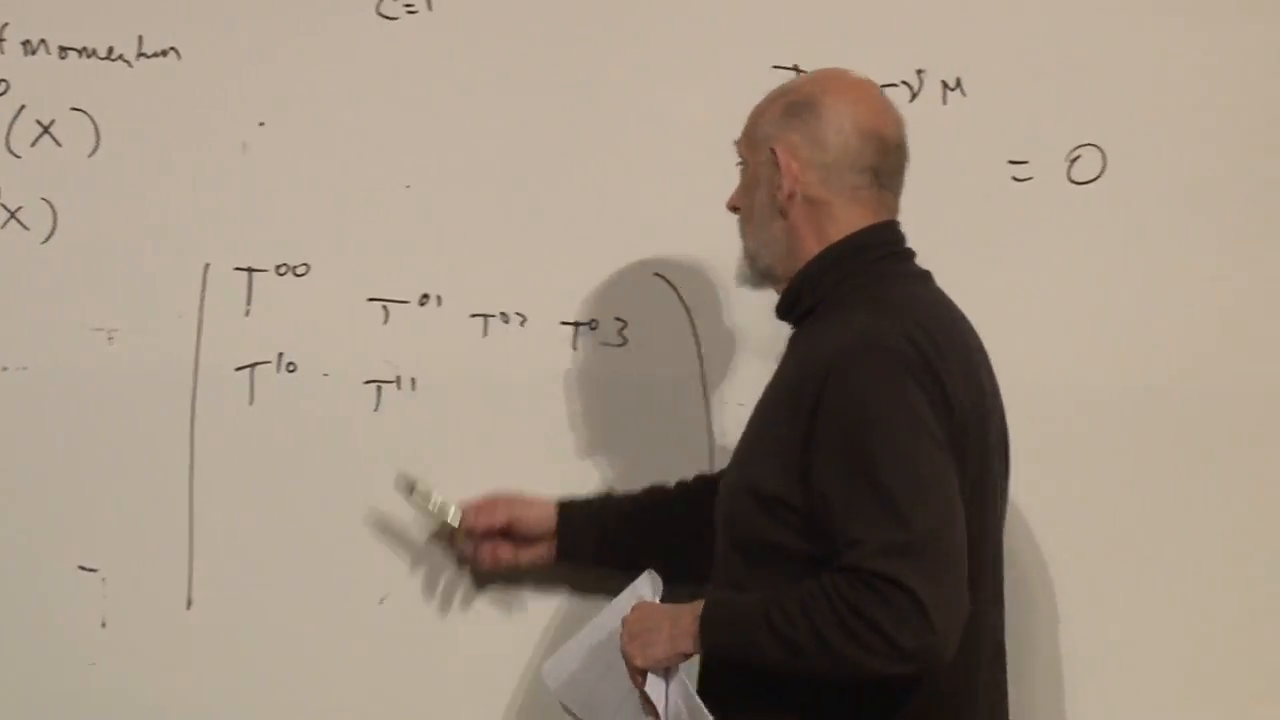
\includegraphics[width=0.84\textwidth]{lecture_09_figure_02.png}
\caption{Der sich entwickelnde Energie-Impuls-Tensor an der Tafel. Der erste Index wählt die Energie oder eine Impulskomponente aus; der zweite die Dichte oder den Fluss.}
\lectureframe{00:44:30}
\end{figure}

Die vollständige Matrix lautet
\begin{equation}
 T^{\mu\nu}=
 \begin{pmatrix}
 T^{00}&T^{01}&T^{02}&T^{03}\\
 T^{10}&T^{11}&T^{12}&T^{13}\\
 T^{20}&T^{21}&T^{22}&T^{23}\\
 T^{30}&T^{31}&T^{32}&T^{33}
 \end{pmatrix}.
\end{equation}
Ein weiterer Satz der relativistischen Mechanik und Feldtheorie besagt, dass der Energie-Impuls-Tensor für die Gravitation symmetrisch ist:
\begin{equation}
 T^{\mu\nu}=T^{\nu\mu}.
 \label{eq:stress-symmetry}
\end{equation}
Insbesondere sind Energiefluss und Impulsdichte die entsprechenden Nebendiagonaleinträge, von gegenüberliegenden Seiten betrachtet. Dank der Symmetrie können wir Gleichung~\eqref{eq:stress-continuity} auch in der vertrauten Form schreiben:
\begin{equation}
 D_\mu T^{\mu\nu}=0.
 \label{eq:stress-conservation}
\end{equation}

\begin{classroomqa}
\audiencequestion{Warum erhielt der Energie-Impuls-Tensor einen zusätzlichen Index, während der Ladungsstrom nur einen benötigt?}
\lecturerresponse{Der Index des Stroms unterscheidet bereits zwischen Dichte und Flussrichtung. Die Ladung benötigt keine zusätzliche Kennzeichnung, weil die erhaltene Ladung ein Skalar ist. Energie und die drei Impulskomponenten sind selbst vier Komponenten; daher gibt der erste Index an, um welche erhaltene Größe es geht, und der zweite, ob es sich um eine Dichte oder einen Fluss handelt.
\lecturetimestamp{00:45:31--00:47:24}}
\end{classroomqa}

\begin{classroomqa}
\audiencequestion{Ist die gesamte Matrix \(T^{\mu\nu}\) symmetrisch und nicht nur die Einträge für Energiefluss und Impulsdichte?}
\lecturerresponse{Ja. Die gesamte Matrix ist symmetrisch. Die genaue Bedeutung ihrer räumlichen Einträge, einschließlich Druck und Spannung, wird später erläutert.
\lecturetimestamp{00:47:32--00:47:54}}
\end{classroomqa}

Die Energiedichte war also nur ein Teil eines umfassenderen Objekts. Als Quelle der Gravitation kann konsistenterweise nicht allein \(T^{00}\) dienen; es muss der vollständige Tensor berücksichtigt werden.

\section{Ein Gesetz kann keine einzelne Komponente auswählen}

Dass eine Tensorgleichung erforderlich ist, lässt sich ohne jede Krümmungsrechnung erkennen. Angenommen, \(A_i\) und \(B_i\) sind Vektoren und ein vorgeschlagenes Gesetz besagt lediglich \(A_3=B_3\). Soll diese Gleichheit in jedem gedrehten Bezugssystem gelten, dreht man die dritte Achse auf die zweite. Dasselbe Gesetz besagt dann \(A_2=B_2\); eine weitere Drehung ergibt \(A_1=B_1\). Ein bezugssystemunabhängiges Gesetz war in Wirklichkeit die Vektorgleichung
\begin{equation}
 A_i=B_i.
\end{equation}

Lorentz-Transformationen erweitern dieselbe Argumentation auf die Zeit. Soll \(A^0=B^0\) in jedem Inertialsystem gelten, mischen Lorentz-Boosts die Zeitkomponente mit den räumlichen Komponenten und erzwingen die vollständige Gleichung \(A^\mu=B^\mu\). Gute relativistische Gesetze müssen Tensoren desselben Typs gleichsetzen.

Die Newtonsche Merkhilfe hob \(T^{00}\) hervor, aber die relativistische Gleichung muss die Form
\begin{equation}
 G_{\mu\nu}=8\pi G\,T_{\mu\nu},
 \label{eq:field-schematic}
\end{equation}
haben, wobei das Symbol \(G_{\mu\nu}\) zunächst nur ein Platzhalter ist. Die erforderlichen Eigenschaften sind nun klar:
\begin{enumerate}
 \item muss ein symmetrischer Tensor zweiter Stufe sein;
 \item muss aus der Metrik gebildet werden, nicht aus Materie;
 \item sollte zwei Ableitungen der Metrik enthalten;
 \item muss seine kovariante Divergenz verschwinden.
\end{enumerate}
Die letzte Bedingung folgt aus Gleichung~\eqref{eq:stress-conservation}.

\section{Suche unter den Krümmungstensoren}

Die Christoffel-Symbole enthalten eine Ableitung der Metrik:
\begin{equation}
 \Gamma^\sigma_{\tau\nu}
 =
 \frac12 g^{\sigma\delta}
 \left(
 \partial_\tau g_{\delta\nu}
 +\partial_\nu g_{\delta\tau}
 -\partial_\delta g_{\tau\nu}
 \right).
 \label{eq:christoffel}
\end{equation}
Sie sind keine Tensoren und können daher nicht selbst die linke Seite liefern. Der Riemann-Krümmungstensor ist ein Tensor:
\begin{equation}
 R^\rho{}_{\sigma\mu\nu}
 =
 \partial_\mu\Gamma^\rho_{\nu\sigma}
 -\partial_\nu\Gamma^\rho_{\mu\sigma}
 +\Gamma^\rho_{\mu\lambda}\Gamma^\lambda_{\nu\sigma}
 -\Gamma^\rho_{\nu\lambda}\Gamma^\lambda_{\mu\sigma}.
 \label{eq:riemann}
\end{equation}
Seine ersten beiden Terme enthalten zweite Ableitungen der Metrik; seine letzten beiden enthalten Produkte erster Ableitungen. Das ist genau die Differentialordnung, die die Newtonsche Gleichung nahelegt.

Das Problem liegt in der Indexstruktur. \(R^\rho{}_{\sigma\mu\nu}\) hat vier Indizes, während \(T_{\mu\nu}\) zwei hat. Durch Kontraktion eines passenden oberen und unteren Index erhält man den Ricci-Tensor,
\begin{equation}
 R_{\mu\nu}=R^\lambda{}_{\mu\lambda\nu}.
 \label{eq:ricci}
\end{equation}
Andere scheinbare Kontraktionen verschwinden entweder aufgrund der Symmetrien des Riemann-Tensors oder ergeben bis auf ein Vorzeichen und die Indexkonvention dasselbe Objekt. Der Ricci-Tensor ist symmetrisch, enthält aber weniger Information als der vollständige Riemann-Tensor: Er kann verschwinden, während der Riemann-Tensor ungleich null bleibt.

\begin{classroomqa}
\audiencequestion{Kann man einfach zwei untere Indizes des Riemann-Tensors kontrahieren? Erfordert eine Kontraktion nicht einen kovarianten und einen kontravarianten Index?}
\lecturerresponse{Genau. Zunächst muss ein Index mit der inversen Metrik angehoben werden, oder gleichbedeutend muss die Kontraktion \(g^{\mu\nu}\) enthalten. In der Schreibweise \(R^\lambda{}_{\mu\lambda\nu}\) ist das erforderliche Paar aus einem oberen und einem unteren Index ausdrücklich zu sehen.
\lecturetimestamp{01:00:09--01:00:33}}
\end{classroomqa}

Eine erneute Kontraktion des Ricci-Tensors ergibt den Krümmungsskalar,
\begin{equation}
 R=g^{\mu\nu}R_{\mu\nu}.
 \label{eq:ricci-scalar}
\end{equation}
Die Multiplikation dieses Skalars mit \(g_{\mu\nu}\) ergibt einen weiteren symmetrischen Tensor zweiter Stufe. Damit haben wir zwei naheliegende Kandidaten gefunden:
\begin{equation}
 R_{\mu\nu},
 \qquad
 g_{\mu\nu}R.
\end{equation}

\begin{figure}[htbp]
\centering
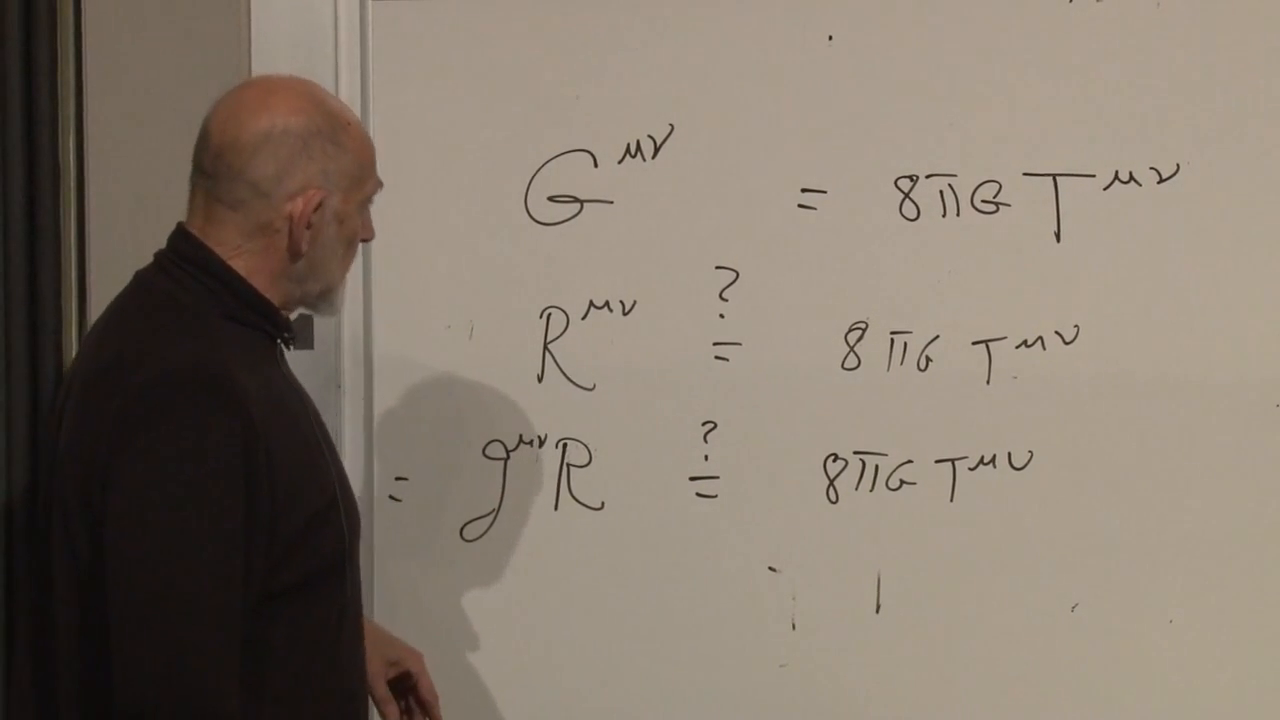
\includegraphics[width=0.78\textwidth]{lecture_09_figure_03.png}
\caption{Die beiden versuchsweise angesetzten geometrischen Tensoren an der Tafel. Zu diesem Zeitpunkt haben beide den richtigen Rang und die richtige Differentialordnung; daher steht jeweils ein Fragezeichen daneben.}
\lectureframe{01:04:56}
\end{figure}

Die vorläufigen Möglichkeiten lauten
\begin{align}
 R_{\mu\nu}&\stackrel{?}{=}8\pi G\,T_{\mu\nu},\\
 g_{\mu\nu}R&\stackrel{?}{=}8\pi G\,T_{\mu\nu}.
\end{align}
Keiner der beiden Ansätze ist allein deshalb anzunehmen, weil seine Indizes passen. Der Erhaltungssatz liefert die entscheidende Prüfung.

\section{Die Prüfung durch die Divergenz}

Wenn Gleichung~\eqref{eq:field-schematic} richtig ist, muss identisch
\begin{equation}
 D_\mu G^{\mu\nu}=0
\end{equation}
gelten, denn \(D_\mu T^{\mu\nu}=0\). Betrachten wir zunächst den Kandidaten mit dem Krümmungsskalar. Die Produktregel ergibt
\begin{equation}
 D_\mu\!\left(g^{\mu\nu}R\right)
 =
 \left(D_\mu g^{\mu\nu}\right)R
 +g^{\mu\nu}D_\mu R.
 \label{eq:product-rule}
\end{equation}

\begin{figure}[htbp]
\centering
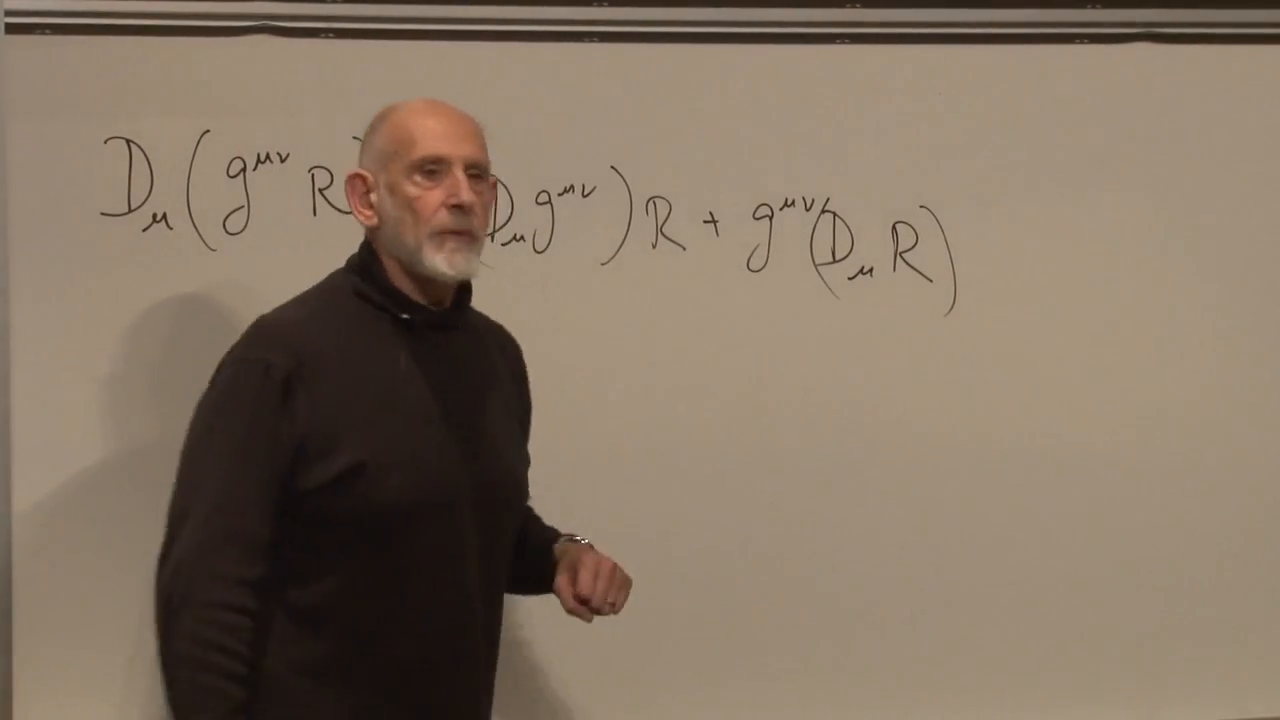
\includegraphics[width=0.84\textwidth]{lecture_09_figure_04.png}
\caption{Anwendung der kovarianten Produktregel auf \(D_\mu(g^{\mu\nu}R)\).}
\lectureframe{01:07:12}
\end{figure}

Die Metrikverträglichkeit besagt:
\begin{equation}
 D_\mu g^{\alpha\beta}=0.
 \label{eq:metric-compatibility}
\end{equation}
Dies ist eine unabhängige geometrische Eigenschaft der Levi-Civita-Verbindung und keine Folge der Energie-Impuls-Erhaltung. Da \(R\) ein Skalar ist, gilt \(D_\mu R=\partial_\mu R\). Gleichung~\eqref{eq:product-rule} wird daher zu
\begin{equation}
 D_\mu(g^{\mu\nu}R)
 =g^{\mu\nu}\partial_\mu R
 =D^\nu R,
\end{equation}
was im Allgemeinen nicht null ist. Der Kandidat \(g^{\mu\nu}R\) scheidet aus.

Die entsprechende Rechnung für den Ricci-Tensor ist etwas länger. Ihr Ergebnis ist die kontrahierte Bianchi-Identität,
\begin{equation}
 D_\mu R^{\mu\nu}=\frac12 D^\nu R.
 \label{eq:contracted-bianchi}
\end{equation}
Damit scheidet auch \(R^{\mu\nu}\) allein aus. Doch die beiden Abweichungen haben genau das Verhältnis, das für ihre Aufhebung erforderlich ist:
\begin{equation}
 D_\mu\left(
 R^{\mu\nu}-\frac12 g^{\mu\nu}R
 \right)=0.
\end{equation}
Dies bestimmt den Einstein-Tensor,
\begin{equation}
 \boxed{
 G_{\mu\nu}
 =
 R_{\mu\nu}-\frac12 g_{\mu\nu}R
 }.
 \label{eq:einstein-tensor}
\end{equation}

Unter den hier geltenden Annahmen -- ein lokaler symmetrischer Tensor zweiter Stufe, der aus der Metrik gebildet wird und höchstens zwei Ableitungen enthält -- ist diese Kombination bis auf einen Gesamtfaktor und einen möglichen Metrikterm eindeutig festgelegt. Letzterer entspricht der Möglichkeit einer kosmologischen Konstante, auf die wir gegen Ende der Vorlesung zurückkommen. Der Koeffizient vor Gleichung~\eqref{eq:einstein-tensor} wird durch den Abgleich mit der Newtonschen Gravitation bestimmt.

\begin{classroomqa}
\audiencequestion{Gibt es einen direkter an die Physik anknüpfenden Weg zur Feldgleichung, statt Kandidaten aufzustellen und sie mithilfe der Kontinuitätsgleichung zu verwerfen?}
\lecturerresponse{Die lokale Erhaltung ist bereits ein physikalisches Prinzip: Energie und Impuls können nicht aus einem Gebiet verschwinden, ohne dessen Grenze zu überqueren. Außerdem gibt es eine kürzere Herleitung aus einem Wirkungsprinzip für das Gravitationsfeld. Die Variation dieser Wirkung ergibt dieselbe Gleichung, auch wenn die Rechnung selbst nicht kurz ist.
\lecturetimestamp{01:17:14--01:18:41}}
\end{classroomqa}

\begin{classroomqa}
\audiencequestion{Könnte ein anderer geometrischer Tensor zweiter Stufe dasselbe Erhaltungsgesetz erfüllen? Ist die Antwort physikalischer oder mathematischer Art, und hätte Einstein sie gekannt?}
\lecturerresponse{Unter den Annahmen dieser Konstruktion ist die Klassifikation mathematischer Art. Die verfügbaren Krümmungsobjekte mit zwei Ableitungen gehen auf den Riemann-Tensor zurück; die beiden gerade geprüften Kandidaten zweiter Stufe umfassen alle relevanten Kontraktionen. Um ihre divergenzfreie Kombination zu finden, ist dennoch eine Rechnung nötig. Die Prinzipien sind einfach, aber die Indizes und Vorzeichen zu handhaben, ist mühsam.
\lecturetimestamp{01:18:42--01:21:44}}
\end{classroomqa}

\section{Die Feldgleichung und ihr Newtonscher Grenzfall}

Die Feldgleichung lautet nun
\begin{equation}
 \boxed{
 R_{\mu\nu}-\frac12 g_{\mu\nu}R
 =
 8\pi G\,T_{\mu\nu}
 }.
 \label{eq:einstein-equation}
\end{equation}
Die linke Seite ist geometrischer Art; die rechte beschreibt Materie, Strahlung und ihre Flüsse. Die kovarianten Divergenzen beider Seiten verschwinden.

Der Faktor \(8\pi G\) wird nicht durch das Divergenzargument bestimmt. Er ergibt sich, indem man ein schwaches, sich langsam änderndes Gravitationsfeld betrachtet, das von langsam bewegter Materie erzeugt wird, und verlangt, dass die Zeit-Zeit-Komponente die Poisson-Gleichung reproduziert. In diesem Regime gilt \(T_{00}\simeq\rho\), während die anderen Komponenten um Potenzen von \(v/c\) unterdrückt sind. Die geometrische Seite nimmt die in Gleichung~\eqref{eq:weak-mnemonic} erwartete Struktur aus zweiten Ableitungen an. Der Abgleich ergibt genau die Normierung in Gleichung~\eqref{eq:einstein-equation}.

Dieser Grenzfall erklärt auch, weshalb die Newtonsche Gravitation scheinbar nur von der Massendichte erzeugt wird. In der vollständigen Theorie trägt jede Komponente von \(T_{\mu\nu}\) zur Gravitation bei: Energiedichte, Energiefluss, Impulsdichte, Druck und Schubspannung. Bei gewöhnlicher nichtrelativistischer Materie dominiert die Ruheenergie. Bei relativistischer Materie, Strahlung oder Systemen mit hohem Druck lassen sich die übrigen Komponenten nicht vernachlässigen.

Der historische Weg war keine mühelose Eingebung. Der Ricci-Tensor wirkt wie der naheliegende erste Ansatz, und der zusätzliche Term \(-\tfrac12g_{\mu\nu}R\) stellt die Vereinbarkeit mit der lokalen Erhaltung wieder her. Sobald die Tensorstruktur feststeht, liefert der Newtonsche Grenzfall die Normierung.

\section{Was bei einer Kontraktion verloren geht}

\begin{classroomqa}
\audiencequestion{Hat die Information, die bei der Kontraktion des Riemann-Tensors von vier auf zwei Indizes verworfen wird, einen physikalischen Gehalt?}
\lecturerresponse{Ja. Der Ricci-Tensor enthält nicht die gesamte Raumzeitkrümmung. Gravitationsfelder ohne Quellen sind die deutlichsten Beispiele: Der Ricci-Tensor kann verschwinden, während Gezeitenkrümmung und Gravitationswellen fortbestehen. Die Kontraktion behält den Teil, der unmittelbar mit der lokalen Quellengleichung zusammenhängt, aber nicht alle Freiheitsgrade des Gravitationsfeldes.
\lecturetimestamp{01:21:57--01:23:10}}
\end{classroomqa}

Die Analogie zur Elektromagnetik ist nützlich. Die Maxwell-Gleichungen erlauben Wellen in einem Gebiet ohne Ladung oder Strom. Ebenso erlaubt Einsteins Gleichung eine nichttriviale Geometrie in einem Gebiet, in dem \(T_{\mu\nu}=0\) gilt. Nun leiten wir die einfachere Gleichung her, die dort gilt.

\section{Vakuum bedeutet Ricci-Flachheit, nicht Flachheit}

Setzen wir
\begin{equation}
 T_{\mu\nu}=0.
\end{equation}
Dann ergibt Gleichung~\eqref{eq:einstein-equation}
\begin{equation}
 R_{\mu\nu}-\frac12g_{\mu\nu}R=0.
 \label{eq:vacuum-einstein}
\end{equation}
Kontraktion mit \(g^{\mu\nu}\). Da
\begin{equation}
 g^{\mu\nu}g_{\mu\nu}
 =\delta^\mu{}_\mu=4
\end{equation}
in vier Raumzeitdimensionen gilt, lautet die Spur
\begin{equation}
 R-\frac12(4)R=-R=0.
\end{equation}
Daher gilt
\begin{equation}
 R=0,
 \qquad
 R_{\mu\nu}=0.
 \label{eq:ricci-flat}
\end{equation}
Die Vakuumfeldgleichung besagt also, dass die Raumzeit Ricci-flach ist.

Es ist entscheidend, \emph{Ricci-flach} nicht durch \emph{flach} zu ersetzen. Im Schwarzschild-Außenraum gibt es abseits der zentralen Singularität keine Materie, und dort gilt \(R_{\mu\nu}=0\). Dennoch ist der Riemann-Tensor ungleich null, und es wirken reale Gezeitenkräfte. Die Ricci-Flachheit lässt sich überprüfen, indem man alle Christoffel-Symbole und Krümmungskomponenten von Hand berechnet, auch wenn das mühsam ist, oder die Buchführung einem Computeralgebrasystem überlässt. An der Singularität divergieren die klassischen Ausdrücke; überall außerhalb davon gilt die Vakuumgleichung.

Gravitationswellen liefern ein zweites Beispiel. Sie können sich durch ein quellenfreies Gebiet ausbreiten und dabei eine echte Verzerrung der Raumzeit mit sich führen. Somit gilt
\begin{equation}
 R_{\mu\nu}=0
 \quad\not\Rightarrow\quad
 R^\rho{}_{\sigma\mu\nu}=0.
\end{equation}

\section{Die Quelle beibehalten: die Spurengleichung}

Die Vorlesung scheint mit dem Vakuumergebnis beinahe zu enden, doch ein Zuhörer bittet darum, die Kontraktion zu wiederholen, ohne die Quelle wegzulassen.

\begin{classroomqa}
\audiencequestion{Was ergibt sich, wenn wir dieselbe Kontraktion durchführen und dabei \(T_{\mu\nu}\) in der Gleichung belassen?}
\lecturerresponse{Die Spur setzt den Krümmungsskalar direkt zur Spur des Energie-Impuls-Tensors in Beziehung. Setzt man diese Beziehung wieder ein, erhält man eine äquivalente Form der Feldgleichung mit dem Ricci-Tensor.
\lecturetimestamp{01:29:28--01:32:20}}
\end{classroomqa}

Definieren wir
\begin{equation}
 T=g^{\mu\nu}T_{\mu\nu}.
\end{equation}
Die Spur von Gleichung~\eqref{eq:einstein-equation} ergibt
\begin{align}
 R-\frac12(4)R&=8\pi G\,T,\\
 -R&=8\pi G\,T,
\end{align}
also
\begin{equation}
 \boxed{R=-8\pi G\,T}.
 \label{eq:trace-relation}
\end{equation}
Einsetzen in die Feldgleichung liefert
\begin{equation}
 \boxed{
 R_{\mu\nu}
 =
 8\pi G
 \left(
 T_{\mu\nu}-\frac12g_{\mu\nu}T
 \right)
 }.
 \label{eq:ricci-form}
\end{equation}

\begin{figure}[htbp]
\centering
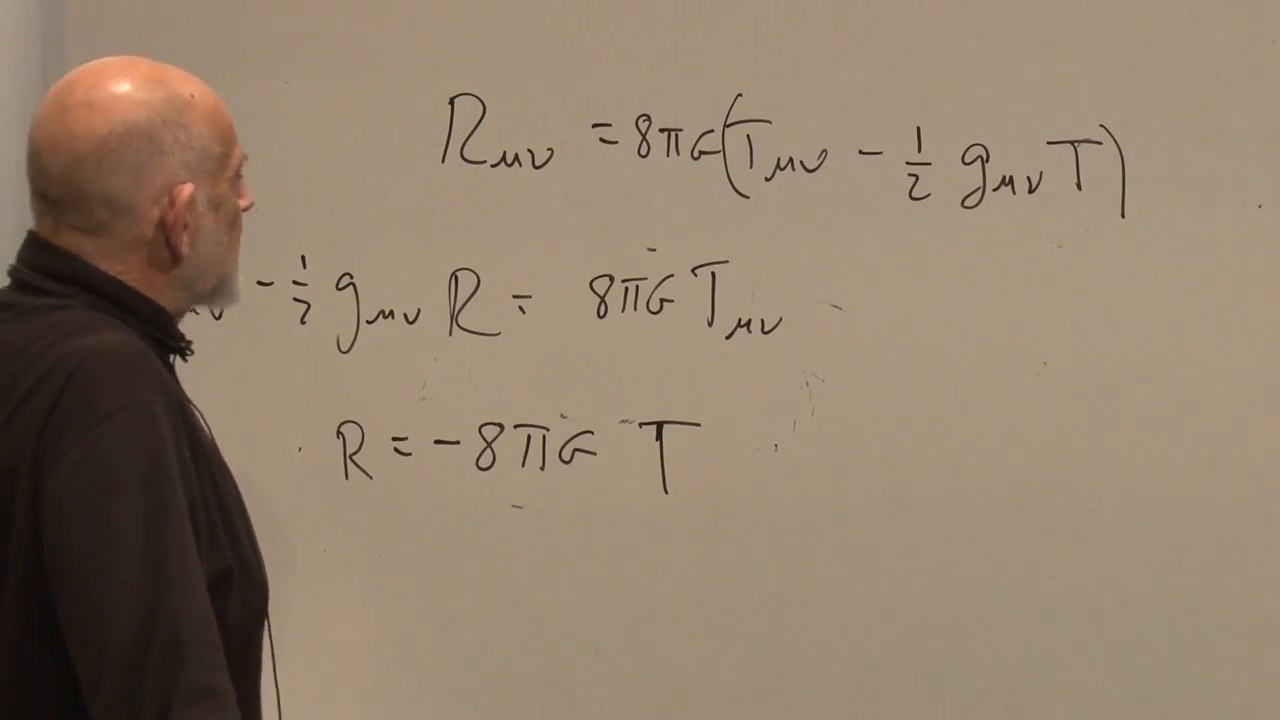
\includegraphics[width=0.82\textwidth]{lecture_09_figure_05.png}
\caption{Die Spurenbeziehung und die äquivalente Form von Einsteins Gleichung mit dem Ricci-Tensor.}
\lectureframe{01:32:25}
\end{figure}

\begin{classroomqa}
\audiencequestion{Hat der Skalar \(T\) eine physikalische Bedeutung?}
\lecturerresponse{Er ist die Spur des Energie-Impuls-Tensors. Für elektromagnetische Strahlung verschwindet sie; dasselbe gilt für ein ideales Gas aus masselosen Teilchen wie Photonen. Massive Materie hat im Allgemeinen eine von null verschiedene Spur. Über Gleichung~\eqref{eq:trace-relation} bestimmt diese Spur den Krümmungsskalar.
\lecturetimestamp{01:32:20--01:33:12}}
\end{classroomqa}

\section{Wie viel Krümmung erfasst der Ricci-Tensor?}

\begin{classroomqa}
\audiencequestion{Gibt es ein einfaches physikalisches oder geometrisches Bild des Ricci-Tensors und des Ricci-Skalars, vergleichbar mit dem Paralleltransport um eine kleine Schleife für den Riemann-Tensor?}
\lecturerresponse{Ein ähnlich anschauliches Bild wird hier nicht angeboten. Der Riemann-Tensor erfasst unmittelbar die Drehung, die beim Transport um eine kleine Schleife entsteht. Seine Kontraktionen sind algebraisch einfacher, doch ihre jeweiligen geometrischen Bedeutungen lassen sich schwerer veranschaulichen. Es ist besser, kein irreführendes Bild zu erfinden, nur weil ein solches praktisch wäre.
\lecturetimestamp{01:33:14--01:34:13}}
\end{classroomqa}

Wie viel Information bei der Kontraktion verloren geht, hängt von der Dimension ab. In vier Dimensionen enthält der Riemann-Tensor Krümmungsinformation, die im Ricci-Tensor nicht vorkommt. In drei Dimensionen ist der Riemann-Tensor durch den Ricci-Tensor bestimmt. In zwei Dimensionen enthält der Krümmungsskalar die gesamte unabhängige Krümmungsinformation. Die vierdimensionale Gravitation lässt daher quellenfreie Krümmungsfreiheitsgrade zu, die in \(R_{\mu\nu}\) nicht sichtbar sind.

\begin{classroomqa}
\audiencequestion{Wenn verschiedene Riemann-Tensoren denselben Ricci-Tensor haben können, wie zeigt sich die fehlende Information physikalisch?}
\lecturerresponse{Eine gegebene Quelle legt für sich genommen nicht jede mögliche Gravitationskonfiguration fest. Rand- und Anfangsdaten können Gravitationsstrahlung enthalten. In der Näherung schwacher Felder kann man sich vorstellen, von einer Lösung mit Quelle auszugehen und eine freie Gravitationswelle hinzuzufügen. Die vollständige nichtlineare Theorie erlaubt keine beliebige Überlagerung, aber das Beispiel veranschaulicht zutreffend die fehlende Information: propagierende Krümmung, die lokal nicht durch \(T_{\mu\nu}\) festgelegt ist.
\lecturetimestamp{01:37:05--01:38:59}}
\end{classroomqa}

Nun fügen sich zwei Vakuumbeispiele zusammen. Die Schwarzschild-Geometrie weist außerhalb einer Masse Gezeitenkrümmung auf. Eine Gravitationswelle trägt sich frei ausbreitende Krümmung. Beide können \(R_{\mu\nu}=0\) erfüllen und dennoch nicht flach sein.

\section{Die kosmologische Konstante}

\begin{classroomqa}
\audiencequestion{Gibt es keinen zusätzlichen Korrekturfaktor, etwa eine kosmologische Konstante?}
\lecturerresponse{Eine kosmologische Konstante ist zulässig. Sie kann auf der geometrischen Seite als Konstante mal \(g_{\mu\nu}\) geschrieben oder auf die rechte Seite gebracht und als Vakuumbeitrag zum Energie-Impuls-Tensor interpretiert werden. Die beiden Beschreibungen sind dieselbe Gleichung mit unterschiedlicher Zuordnung der Terme.
\lecturetimestamp{01:39:01--01:40:44}}
\end{classroomqa}

Mit einer kosmologischen Konstante lautet eine gebräuchliche Konvention
\begin{equation}
 G_{\mu\nu}+\Lambda g_{\mu\nu}
 =
 8\pi G\,T_{\mu\nu}.
\end{equation}
Verschiebt man den zusätzlichen Term auf die rechte Seite, erhält man als Definition einen effektiven Vakuum-Spannungstensor,
\begin{equation}
 T_{\mu\nu}^{(\Lambda)}
 =
 -\frac{\Lambda}{8\pi G}g_{\mu\nu}.
\end{equation}
Da aus der Metrikverträglichkeit \(D_\mu g^{\mu\nu}=0\) folgt, ist der zusätzliche Term automatisch mit dem Erhaltungsgesetz vereinbar. Dies ist der Metrikterm, den die frühere Eindeutigkeitsaussage offengelassen hat.

\section{Merkur und die Schwachfeldrechnung}

\begin{classroomqa}
\audiencequestion{Hat Einstein diese Gleichung verwendet, um die Bahn des Merkur zu berechnen, und wo kann man sehen, wie diese Berechnung durchgeführt wurde?}
\lecturerresponse{Einstein arbeitete, bevor Schwarzschild die exakte Lösung angab, und verwendete stattdessen eine hinreichend genaue Fernfeldnäherung für das Außenfeld der Sonne. Der Sonnenradius und die Merkurbahn sind sehr groß im Vergleich zum Schwarzschildradius der Sonne, sodass relativistische Korrekturen klein sind. Er konnte von einer Keplerbahn ausgehen und die Korrektur störungstheoretisch berechnen. Schwarzschild fand kurz darauf die exakte Außenlösung, wodurch sich dieselbe Berechnung systematisch durchführen ließ.
\lecturetimestamp{01:40:46--01:43:48}}
\end{classroomqa}

Störungstheorie bedeutet genau dies: Man beginnt mit einem bereits gelösten Problem und berechnet anschließend den Einfluss einer kleinen Korrektur. Die Newtonsche Kraft mit umgekehrt quadratischem Abstandsgesetz ergibt geschlossene Kepler-Ellipsen. Die allgemeine Relativitätstheorie fügt der Newtonschen Radialgleichung eine kleine Abweichung hinzu, sodass sich die Ellipse nach einem Umlauf nicht schließt; ihr Perihel verschiebt sich.

Die Vorlesung schließt mit der merkwürdigen Besonderheit geschlossener Bahnen im Zentralfeld. Die Kraft nach dem inversen Quadratgesetz ist insofern außergewöhnlich, als ihre Keplerbahnen ohne Präzession geschlossen sind. Allgemeiner weist Bertrands Theorem auch den isotropen harmonischen Oszillator als das andere Zentralpotential aus, bei dem jede gebundene Bahn geschlossen ist. Die kleine relativistische Korrektur hebt diese Newtonsche Entartung auf und macht die Präzession des Merkur zu einem beobachtbaren Kennzeichen der in diesem Kapitel hergeleiteten Feldgleichung.